\documentclass[t]{beamer}

\usepackage{amsmath}
\usepackage{pgfplots}
\usepackage{soul}
\usepackage{tikz}

\pgfplotsset{compat=1.9}

\usetheme{metropolis}

\author{Esten H{\o}yland Leonardsen}
\institute[Life Science, UiO]{UiO:Life Science, University of Oslo}
\date{02.11.22}
\title{Introduction to deep learning 1/?}

\titlegraphic{
	\vspace*{6.8cm}
	\centering
    
\includegraphics[width=1.5cm]{data/uio.png}
}

\makeatletter
\let\UL\ul
\renewcommand\ul{%
  \let\set@color\beamerorig@set@color
  \let\reset@color\beamerorig@reset@color
  \UL}

\begin{document}

	\def\nodesize{14pt}
	\begin{frame}
		\titlepage
	\end{frame}

	\begin{frame}{Introduction}
		\vfill
		\centering
		\begin{enumerate}
			\item Building an artificial neural network (ANN)
			\item Training the ANN
			\item Transformation to a Convolutional Neural Network (CNN)
		\end{enumerate}
		\vfill
	\end{frame}

	\begin{frame}{Building a neural network: Linear regression}
		\centering
		\vfill
		\begin{tikzpicture}
			\node[] at (-5, 3) {};
			\node[] at (5, -4.5) {};

			\node[] at (0, 0) {$y=ax+b$};
		\end{tikzpicture}
		\vfill
	\end{frame}

	\begin{frame}{Building a neural network: Linear regression}
		\centering
		\vfill
		\begin{tikzpicture}
			\node[] at (-5, 3) {};
			\node[] at (5, -4.5) {};

			\node[] at (0, 0) {$y=ax+b$};

			\draw[] (-2, -1.5) -- (2, -1.5) -- (2, -4) -- (-2, -4) -- (-2, -1.5);

			\draw[very thick, blue!60] (-2, -3.5) -- (2, -1.75);

			\node[anchor=north] at (0, -4.1) {x};
			\node[anchor=south, rotate=90] at (-2.1, -2.75) {y};
		\end{tikzpicture}
		\vfill
	\end{frame}

	\begin{frame}{Building a neural network: Linear regression}
		\centering
		\vfill
		\begin{tikzpicture}
			\node[] at (-5, 3) {};
			\node[] at (5, -4.5) {};

			\node[
				circle,
				draw=black,
				fill=green!20,
				minimum size=\nodesize,
				inner sep=0pt
			] (n) at (0, 1.5) {};
			\node[] (x) at (-1.5, 1.5) {$x$};
			\node[] (b) at (0, 2.5) {$b$};
			\node[] (y) at (1.5, 1.5) {$y$};
			\node[] at (0, 0) {$y=ax+b$};

			\draw[->] (x) -- (n) node [midway, above] {$a$};
			\draw[->] (b) -- (n);
			\draw[->] (n) -- (y);

			\draw[] (-2, -1.5) -- (2, -1.5) -- (2, -4) -- (-2, -4) -- (-2, -1.5);

			\draw[very thick, blue!60] (-2, -3.5) -- (2, -1.75);

			\node[anchor=north] at (0, -4.1) {x};
			\node[anchor=south, rotate=90] at (-2.1, -2.75) {y};
		\end{tikzpicture}
		\vfill
	\end{frame}

	\begin{frame}{Building a neural network: Artificial neuron}
		\centering
		\vfill
		\begin{tikzpicture}
			\node[] at (-5, 3) {};
			\node[] at (5, -4.5) {};

			\node[
				circle,
				draw=black,
				fill=green!20,
				minimum size=\nodesize,
				inner sep=0pt
			] (n) at (0, 1.5) {};
			\node[] (x) at (-1.5, 1.5) {$x$};
			\node[] (b) at (0, 2.5) {$b$};
			\node[] (y) at (1.5, 1.5) {$y$};
			\node[] at (0, 0) {$y=max(0, wx+b)$};

			\draw[->] (x) -- (n) node [midway, above] {$w$};
			\draw[->] (b) -- (n);
			\draw[->] (n) -- (y);

			\draw[] (-2, -1.5) -- (2, -1.5) -- (2, -4) -- (-2, -4) -- (-2, -1.5);
			\draw[very thick, blue!60] (-2, -3.5) -- (0, -3.5) -- (2, -1.75);

			\node[anchor=north] at (0, -4.1) {x};
			\node[anchor=south, rotate=90] at (-2.1, -2.75) {y};
		\end{tikzpicture}
		\vfill
	\end{frame}

	\begin{frame}{Building a neural network: Artificial neural network (ANN)}
		\centering
		\vfill
		\begin{tikzpicture}
			\node[] at (-5, 3) {};
			\node[] at (5, -4.5) {};

			\node[
				circle,
				draw=black,
				fill=green!20,
				minimum size=\nodesize,
				inner sep=0pt
			] (n0) at (0, 2) {};
			\node[
				circle,
				draw=black,
				fill=green!20,
				minimum size=\nodesize,
				inner sep=0pt
			] (n1) at (0, 1) {};
			\node[] (x) at (-1.5, 1.5) {$x$};
			\node[] (y) at (1.5, 1.5) {$y$};
			\node[] at (0, 0) {$y=max(0, w_0x+b_0)+max(0, w_1x+b_1)$};

			\draw[->] (x) -- (n0) node [midway, above] {$w_0$};
			\draw[->] (x) -- (n1) node [midway, below] {$w_1$};
			\draw[->] (n0) -- (y);
			\draw[->] (n1) -- (y);

			\draw[] (-2, -1.5) -- (2, -1.5) -- (2, -4) -- (-2, -4) -- (-2, -1.5);
			\draw[very thick, blue!60] (-2, -3.5) -- (-0.66, -3.5) -- (0.66, -2.25) -- (2, -3);

			\node[anchor=north] at (0, -4.1) {x};
			\node[anchor=south, rotate=90] at (-2.1, -2.75) {y};
		\end{tikzpicture}
		\vfill
	\end{frame}

	\begin{frame}{Building a neural network: Universal approximation theorem}
		\vfill
		\centering
		\begin{quotation}
			\centering
			"Any relationship that can be described with a polynomial function can be approximated by a neural network with a single hidden layer."
		\end{quotation}
		- Some guy in the 80s, probably
		\vfill
	\end{frame}

	\begin{frame}{Building a neural network: Universal approximation theorem}
		\setulcolor{red}
		\vfill
		\centering
		\begin{quotation}
			\centering
			"Any relationship that can be \ul{described with a polynomial function} can be \ul{approximated} by a neural network with a single hidden layer."
		\end{quotation}
		- Some guy in the 80s, probably
		\vfill
	\end{frame}

	\begin{frame}{Building a neural network: Increasing dimensionality}
		\centering
		\vfill
		\newsavebox{\mybox}
		\sbox{\mybox}{%
			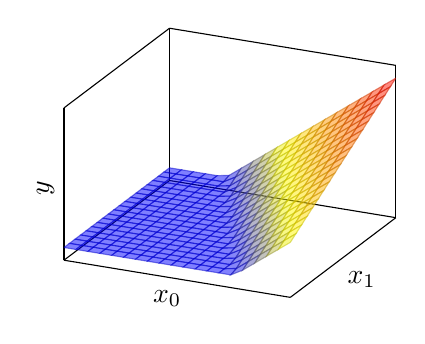
\begin{tikzpicture}[
				declare function = {
					q(\x) = \x - 1;
					Z(\x,\y) = max(0, \x*0.5 + \y*0.25);
				}
			]
				\begin{axis}
				[
					height=5cm,
					ticks=none,
					xlabel=$x_0$,
					ylabel=$x_1$,
					zlabel=$y$,
					domain=-1:1,
					samples=20,
				]
					\addplot3 [surf, opacity=0.5] {Z(x,y)};
				\end{axis}
			\end{tikzpicture}
		}
		\begin{tikzpicture}
			\node[] at (-5, 3) {};
			\node[] at (5, -4.5) {};

			\node[
				circle,
				draw=black,
				fill=green!20,
				minimum size=\nodesize,
				inner sep=0pt
			] (n) at (0, 1.5) {};
			\node[] (x0) at (-1.5, 2) {$x_0$};
			\node[] (x1) at (-1.5, 1) {$x_1$};
			\node[] (b) at (0, 2.5) {$b$};
			\node[] (y) at (1.5, 1.5) {$y$};
			\node[] at (0, 0) {$y=max(0, w_0x_0+w_1x_1+b)$};

			\draw[->] (x0) -- (n) node [midway, above] {$w_0$};
			\draw[->] (x1) -- (n) node [midway, below] {$w_1$};
			\draw[->] (b) -- (n);
			\draw[->] (n) -- (y);

			\node[] at (0, -2.75) {
				\usebox{\mybox}
			};
		\end{tikzpicture}
		\vfill
	\end{frame}

	\begin{frame}{Building a neural network}
		\centering
		\vfill
		\begin{tikzpicture}
			\node[] at (-3.5, 1.25) {};
			\node[] at (3.5, -6.25) {};
			\node[
				circle,
				minimum size=\nodesize,
				inner sep=0pt,
				text depth=0
			] (x) at (-3, 0) {\footnotesize{$x$}};

			\node[
				circle,
				draw=black,
				fill=green!20,
				minimum size=\nodesize,
				inner sep=0pt
			] (n00) at (0, 0.5) {};
			\node[
				circle,
				draw=black,
				fill=green!20,
				minimum size=\nodesize,
				inner sep=0pt
			] (n01) at (0, -0.5) {};

			\node[
				circle,
				minimum size=\nodesize,
				inner sep=0pt,
				text depth=0
			] (y) at (3, 0) {\footnotesize{$y$}};

			\draw[->] (x) -- (n00) node [midway, above] {$w_0$};
			\draw[->] (x) -- (n01) node [midway, below] {$w_1$};

			\draw[->] (n00) -- (y);
			\draw[->] (n01) -- (y);

			\def\spacing{-0.1cm}
			\node[anchor=north] at (0, -1.5) {\tiny{
				\begin{math}
					\begin{alignedat}{5}
						y = max(0, w_0x+b_0)+max(0, w_1x+b_1)\\
					\end{alignedat}
				\end{math}
			}};
		\end{tikzpicture}
		\vfill
	\end{frame}

	\begin{frame}{Building a neural network}
		\centering
		\vfill
		\begin{tikzpicture}
			\node[] at (-3.5, 1.25) {};
			\node[] at (3.5, -6.25) {};
			\node[
				circle,
				draw=black,
				fill=green!20,
				minimum size=\nodesize,
				inner sep=0pt,
				text depth=0
			] (x) at (-3, 0) {\footnotesize{$x$}};

			\node[
				circle,
				draw=black,
				fill=green!20,
				minimum size=\nodesize,
				inner sep=0pt
			] (n00) at (0, 0.5) {};
			\node[
				circle,
				draw=black,
				fill=green!20,
				minimum size=\nodesize,
				inner sep=0pt
			] (n01) at (0, -0.5) {};

			\node[
				circle,
				draw=black,
				fill=green!20,
				minimum size=\nodesize,
				inner sep=0pt,
				text depth=0
			] (y) at (3, 0) {\footnotesize{$y$}};

			\draw[->] (x) -- (n00) node [midway, above] {$w^0_0$};
			\draw[->] (x) -- (n01) node [midway, below] {$w^0_1$};

			\draw[->] (n00) -- (y) node [midway, above] {$w^1_0$};
			\draw[->] (n01) -- (y) node [midway, below] {$w^1_0$};

			\def\spacing{-0.1cm}
			\node[anchor=north] at (0, -1.5) {\tiny{
				\begin{math}
					\begin{alignedat}{5}
						y = max(0, w^1_{0,0}*max(0, w^0_{0,0}*x+b_{0,0})+w^1_{1,0}*max(0, w^0_{0,1}*x+b_{1,0})+b_1)\\
					\end{alignedat}
				\end{math}
			}};
		\end{tikzpicture}
		\vfill
	\end{frame}

	\begin{frame}{Building a neural network}
		\centering
		\vfill
		\begin{tikzpicture}
			\node[] at (-3.5, 1.25) {};
			\node[] at (3.5, -6.25) {};
			\node[
				circle,
				draw=black,
				fill=green!20,
				minimum size=\nodesize,
				inner sep=0pt,
				text depth=0
			] (x) at (-3, 0) {\footnotesize{$x$}};

			\node[
				circle,
				draw=black,
				fill=green!20,
				minimum size=\nodesize,
				inner sep=0pt
			] (n00) at (0, 0.5) {};
			\node[
				circle,
				draw=black,
				fill=green!20,
				minimum size=\nodesize,
				inner sep=0pt
			] (n01) at (0, -0.5) {};

			\node[
				circle,
				draw=black,
				fill=green!20,
				minimum size=\nodesize,
				inner sep=0pt,
				text depth=0
			] (y) at (3, 0) {\footnotesize{$y$}};

			\node[text depth=0] at (-3, -1.2) {\textcolor{red}{Input}};
			\node[text depth=0] at (0, -1.2) {\textcolor{red}{Hidden}};
			\node[text depth=0] at (3, -1.2) {\textcolor{red}{Output}};

			\draw[->] (x) -- (n00) node [midway, above] {$w^0_0$};
			\draw[->] (x) -- (n01) node [midway, below] {$w^0_1$};

			\draw[->] (n00) -- (y) node [midway, above] {$w^1_0$};
			\draw[->] (n01) -- (y) node [midway, below] {$w^1_0$};

			\def\spacing{-0.1cm}
			\node[anchor=north] at (0, -1.5) {\tiny{
				\begin{math}
					\begin{alignedat}{5}
						y = max(0, w^1_{0,0}*max(0, w^0_{0,0}*x+b_{0,0})+w^1_{1,0}*max(0, w^0_{0,1}*x+b_{1,0})+b_1)\\
					\end{alignedat}
				\end{math}
			}};
		\end{tikzpicture}
		\vfill
	\end{frame}

	\begin{frame}{Building a neural network}
		\centering
		\vfill
		\begin{tikzpicture}
			\node[] at (-3.5, 1.25) {};
			\node[] at (3.5, -6.25) {};
			\node[
				circle,
				draw=black,
				fill=green!20,
				minimum size=\nodesize,
				inner sep=0pt,
				text depth=0
			] (x0) at (-3, 0.5) {\footnotesize{$x_0$}};
			\node[
				circle,
				draw=black,
				fill=green!20,
				minimum size=\nodesize,
				inner sep=0pt,
				text depth=0
			] (x1) at (-3, -0.5) {\footnotesize{$x_1$}};

			\node[
				circle,
				draw=black,
				fill=green!20,
				minimum size=\nodesize,
				inner sep=0pt
			] (n00) at (0, 0.5) {};
			\node[
				circle,
				draw=black,
				fill=green!20,
				minimum size=\nodesize,
				inner sep=0pt
			] (n01) at (0, -0.5) {};

			\node[
				circle,
				draw=black,
				fill=green!20,
				minimum size=\nodesize,
				inner sep=0pt,
				text depth=0
			] (y) at (3, 0) {\footnotesize{$y$}};

			\draw[->] (x0) -- (n00);
			\draw[->] (x0) -- (n01);
			\draw[->] (x1) -- (n00);
			\draw[->] (x1) -- (n01);

			\draw[->] (n00) -- (y);
			\draw[->] (n01) -- (y);

			\def\spacing{-0.1cm}
			\node[anchor=north] at (0, -1.5) {\tiny{
				\begin{math}
					\begin{alignedat}{5}
						y &= max(0, &&w^1_{0,0}*max(0, w^0_{0,0}*x_0+w^0_{1,0}*x_{1}+b_{0,0})+\\[\spacing]
						& &&w^1_{1,0}*max(0, w^0_{0,1}*x_0+w^0_{1,1}*x_{1}+b_{0,1})+\\[\spacing]
						& &&b_1)&&\\
					\end{alignedat}
				\end{math}
			}};
		\end{tikzpicture}
		\vfill
	\end{frame}

	\begin{frame}{Building a neural network}
		\centering
		\vfill
		\begin{tikzpicture}
			\node[] at (-3.5, 1.25) {};
			\node[] at (3.5, -6.25) {};
			\node[
				circle,
				draw=black,
				fill=green!20,
				minimum size=\nodesize,
				inner sep=0pt,
				text depth=0
			] (x0) at (-3, 0.5) {\footnotesize{$x_0$}};
			\node[
				circle,
				draw=black,
				fill=green!20,
				minimum size=\nodesize,
				inner sep=0pt,
				text depth=0
			] (x1) at (-3, -0.5) {\footnotesize{$x_1$}};

			\node[
				circle,
				draw=black,
				fill=green!20,
				minimum size=\nodesize,
				inner sep=0pt
			] (n00) at (0, 1) {};
			\node[
				circle,
				draw=black,
				fill=green!20,
				minimum size=\nodesize,
				inner sep=0pt
			] (n01) at (0, 0) {};
			\node[
				circle,
				draw=black,
				fill=green!20,
				minimum size=\nodesize,
				inner sep=0pt
			] (n02) at (0, -1) {};

			\node[
				circle,
				draw=black,
				fill=green!20,
				minimum size=\nodesize,
				inner sep=0pt,
				text depth=0
			] (y) at (3, 0) {\footnotesize{$y$}};

			\draw[->] (x0) -- (n00);
			\draw[->] (x0) -- (n01);
			\draw[->] (x0) -- (n02);
			\draw[->] (x1) -- (n00);
			\draw[->] (x1) -- (n01);
			\draw[->] (x1) -- (n02);

			\draw[->] (n00) -- (y);
			\draw[->] (n01) -- (y);
			\draw[->] (n02) -- (y);

			\def\spacing{-0.1cm}
			\node[anchor=north] at (0, -1.5) {\tiny{
				\begin{math}
					\begin{alignedat}{5}
						y &= max(0, &&w^1_{0,0}*max(0, w^0_{0,0}*x_0+w^0_{1,0}*x_{1}+b_{0,0})+\\[\spacing]
						& &&w^1_{1,0}*max(0, w^0_{0,1}*x_0+w^0_{1,1}*x_{1}+b_{0,1})+\\[\spacing]
						& &&w^1_{2,0}*max(0, w^0_{0,2}*x_0+w^0_{1,2}*x_{1}+b_{0,2})+\\[\spacing]
						& &&b_1)&&\\
					\end{alignedat}
				\end{math}
			}};
		\end{tikzpicture}
		\vfill
	\end{frame}

	\begin{frame}{Building a neural network}
		\centering
		\vfill
		\begin{tikzpicture}
			\node[] at (-3.5, 1.25) {};
			\node[] at (3.5, -6.25) {};
			\node[
				circle,
				draw=black,
				fill=green!20,
				minimum size=\nodesize,
				inner sep=0pt,
				text depth=0
			] (x0) at (-3, 0.5) {\footnotesize{$x_0$}};
			\node[
				circle,
				draw=black,
				fill=green!20,
				minimum size=\nodesize,
				inner sep=0pt,
				text depth=0
			] (x1) at (-3, -0.5) {\footnotesize{$x_1$}};

			\node[
				circle,
				draw=black,
				fill=green!20,
				minimum size=\nodesize,
				inner sep=0pt
			] (n00) at (-1, 1) {};
			\node[
				circle,
				draw=black,
				fill=green!20,
				minimum size=\nodesize,
				inner sep=0pt
			] (n01) at (-1, 0) {};
			\node[
				circle,
				draw=black,
				fill=green!20,
				minimum size=\nodesize,
				inner sep=0pt
			] (n02) at (-1, -1) {};

			\node[
				circle,
				draw=black,
				fill=green!20,
				minimum size=\nodesize,
				inner sep=0pt
			] (n10) at (1, 1) {};

			\node[
				circle,
				draw=black,
				fill=green!20,
				minimum size=\nodesize,
				inner sep=0pt
			] (n11) at (1, 0) {};
			\node[
				circle,
				draw=black,
				fill=green!20,
				minimum size=\nodesize,
				inner sep=0pt
			] (n12) at (1, -1) {};

			\node[
				circle,
				draw=black,
				fill=green!20,
				minimum size=\nodesize,
				inner sep=0pt,
				text depth=0
			] (y) at (3, 0) {\footnotesize{$y$}};

			\draw[->] (x0) -- (n00);
			\draw[->] (x0) -- (n01);
			\draw[->] (x0) -- (n02);
			\draw[->] (x1) -- (n00);
			\draw[->] (x1) -- (n01);
			\draw[->] (x1) -- (n02);

			\draw[->] (n00) -- (n10);
			\draw[->] (n00) -- (n11);
			\draw[->] (n00) -- (n12);
			\draw[->] (n01) -- (n10);
			\draw[->] (n01) -- (n11);
			\draw[->] (n01) -- (n12);
			\draw[->] (n02) -- (n10);
			\draw[->] (n02) -- (n11);
			\draw[->] (n02) -- (n12);

			\draw[->] (n10) -- (y);
			\draw[->] (n11) -- (y);
			\draw[->] (n12) -- (y);

			\def\spacing{-0.1cm}
			\node[anchor=north] at (0, -1.5) {\tiny{
				\begin{math}
					\begin{alignedat}{5}
						y &= max(0, &&w^2_{0,0}*max(0, &&w^1_{0,0}*max(0, w^0_{0,0}*x_0+w^0_{1,0}*x_{1}+b_{0,0})+\\[\spacing]
						& && &&w^1_{1,0}*max(0, w^0_{0,1}*x_0+w^+_{1,1}*w_{1}+b_{0,1})+\\[\spacing]
						& && &&w^1_{2,0}*max(0, w^0_{0,2}*x_0+w^+_{1,2}*w_{1}+b_{0,2})+\\[\spacing]
						& && &&b_{1,0})+\\[\spacing]
						& &&w^2_{1,0}*max(0, &&w^1_{0,1}*max(0, w^0_{0,0}*x_0+w^0_{1,0}*x_{1}+b_{0,0})+\\[\spacing]
						& && &&w^1_{1,1}*max(0, w^0_{0,1}*x_0+w^+_{1,1}*w_{1}+b_{0,1})+\\[\spacing]
						& && &&w^1_{2,1}*max(0, w^0_{0,2}*x_0+w^+_{1,2}*w_{1}+b_{0,2})+\\[\spacing]
						& && &&b_{1,1})+\\[\spacing]
						& &&w^2_{2,0}*max(0, &&w^1_{0,2}*max(0, w^0_{0,0}*x_0+w^0_{1,0}*x_{1}+b_{0,0})+\\[\spacing]
						& && &&w^1_{1,2}*max(0, w^0_{0,1}*x_0+w^+_{1,1}*w_{1}+b_{0,1})+\\[\spacing]
						& && &&w^1_{2,2}*max(0, w^0_{0,2}*x_0+w^+_{1,2}*w_{1}+b_{0,2})+\\[\spacing]
						& && &&b_{1,2})+\\[\spacing]
						& &&b_2)&&\\
					\end{alignedat}
				\end{math}
			}};
		\end{tikzpicture}
		\vfill
	\end{frame}

	\begin{frame}{Building a neural network: Summary}
		\centering
		\vfill
		\begin{itemize}
			\item Artificial neurons are (linear) weighted sums wrapped in non-linear activation functions
			\item Multiple artificial neurons stacked together in a layerwise fashion comprise an artificial neural network
			\item Artificial neural networks allow us to model arbitrarily complex relationships between inputs and outputs
		\end{itemize}
		\vfill
	\end{frame}

	\begin{frame}{Training a neural network: Loss functions}
		\newsavebox{\boxseven}
		\sbox{\boxseven}{%
			\begin{tikzpicture}
				\begin{axis}[
					xmin=0,
					xmax=1,
					ymin=0,
					ymax=1,
					ticks=none,
					xlabel=Age,
					ylabel=Height,
					height=0.55\textwidth,
					width=0.8\textwidth
				]

					\addplot[only marks, draw=black, fill=red!60, mark size=3pt] coordinates {
						(0.15, 0.3)
						(0.25, 0.2)
						(0.3, 0.4)
						(0.5, 0.4)
						(0.75, 0.8)
						(0.8, 0.6)
					};
				\end{axis}
			\end{tikzpicture}
		}
		\begin{tikzpicture}
			\node[] at (-5.3, 2.5) {};
			\node[] at (5.3, -5) {};
			\node[] at (0, 0) {
				\usebox{\boxseven}
			};
		\end{tikzpicture}
	\end{frame}

	\begin{frame}{Training a neural network: Loss functions}
		\newsavebox{\boxsix}
		\sbox{\boxsix}{%
			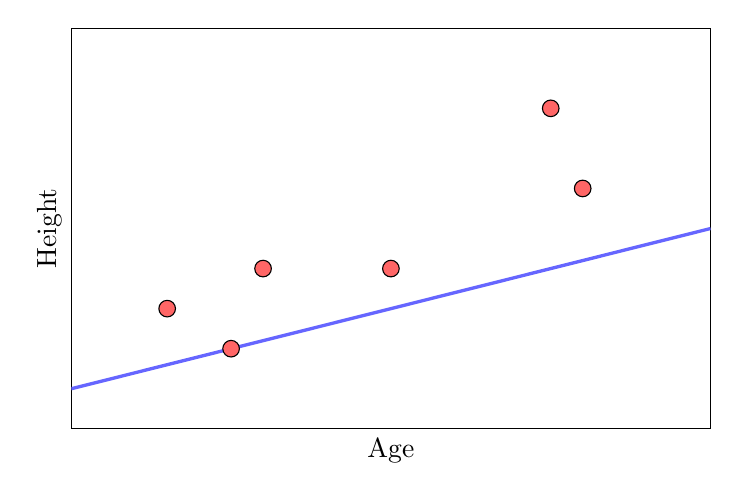
\begin{tikzpicture}
				\begin{axis}[
					xmin=0,
					xmax=1,
					ymin=0,
					ymax=1,
					ticks=none,
					xlabel=Age,
					ylabel=Height,
					height=0.55\textwidth,
					width=0.8\textwidth
				]

					\addplot[only marks, draw=black, fill=red!60, mark size=3pt] coordinates {
						(0.15, 0.3)
						(0.25, 0.2)
						(0.3, 0.4)
						(0.5, 0.4)
						(0.75, 0.8)
						(0.8, 0.6)
					};
					\addplot[blue!60, very thick] coordinates {
						(0, 0.1)
						(1, 0.5)
					};
				\end{axis}
			\end{tikzpicture}
		}
		\begin{tikzpicture}
			\node[] at (-5.3, 2.5) {};
			\node[] at (5.3, -5) {};
			\node[] at (0, 0) {
				\usebox{\boxsix}
			};
			\node[anchor=north] at (0, -2.5) {
				\begin{math}
					\begin{alignedat}{2}
						\hat{y} &= 0.4x + 0.1\\
					\end{alignedat}
				\end{math}
			};
		\end{tikzpicture}
	\end{frame}

	\begin{frame}{Training a neural network: Loss functions}
		\newsavebox{\boxfive}
		\sbox{\boxfive}{%
			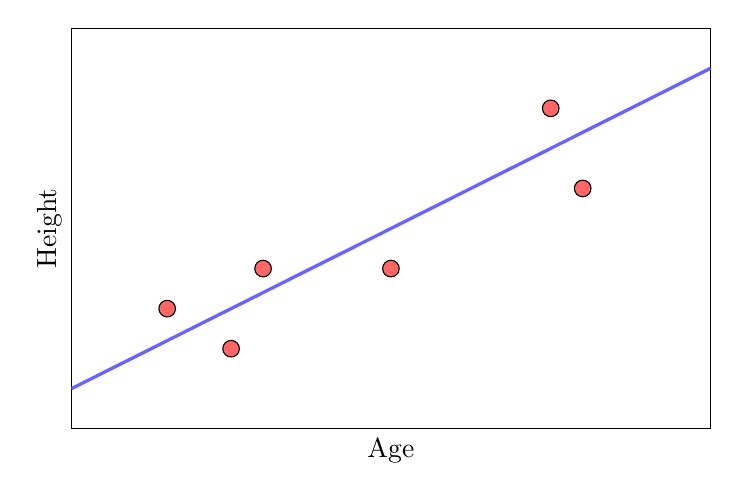
\begin{tikzpicture}
				\begin{axis}[
					xmin=0,
					xmax=1,
					ymin=0,
					ymax=1,
					ticks=none,
					xlabel=Age,
					ylabel=Height,
					height=0.55\textwidth,
					width=0.8\textwidth
				]

					\addplot[only marks, draw=black, fill=red!60, mark size=3pt] coordinates {
						(0.15, 0.3)
						(0.25, 0.2)
						(0.3, 0.4)
						(0.5, 0.4)
						(0.75, 0.8)
						(0.8, 0.6)
					};
					\addplot[blue!60, very thick] coordinates {
						(0, 0.1)
						(1, 0.9)
					};
				\end{axis}
			\end{tikzpicture}
		}
		\begin{tikzpicture}
			\node[] at (-5.3, 2.5) {};
			\node[] at (5.3, -5) {};
			\node[] at (0, 0) {
				\usebox{\boxfive}
			};
			\node[anchor=north] at (0, -2.5) {
				\begin{math}
					\begin{alignedat}{2}
						\hat{y} &= 0.9x + 0.1\\
					\end{alignedat}
				\end{math}
			};
		\end{tikzpicture}
	\end{frame}

	\begin{frame}{Training a neural network: Loss functions}
		\newsavebox{\boxfour}
		\sbox{\boxfour}{%
			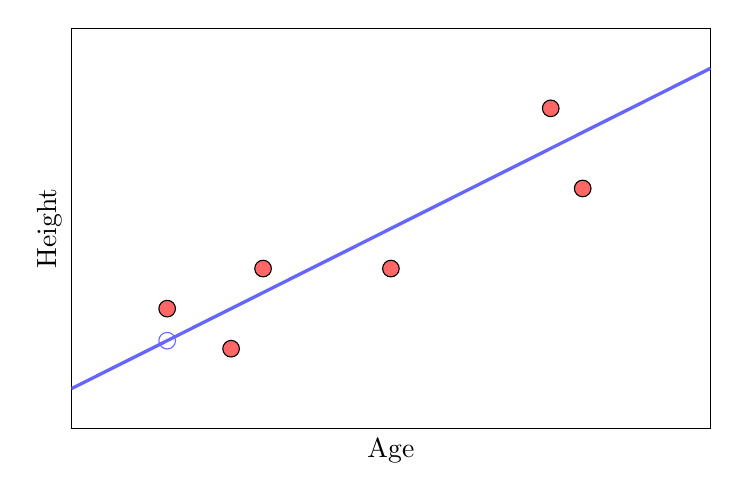
\begin{tikzpicture}
				\begin{axis}[
					xmin=0,
					xmax=1,
					ymin=0,
					ymax=1,
					ticks=none,
					xlabel=Age,
					ylabel=Height,
					height=0.55\textwidth,
					width=0.8\textwidth
				]

					\addplot[only marks, draw=black, fill=red!60, mark size=3pt] coordinates {
						(0.15, 0.3)
						(0.25, 0.2)
						(0.3, 0.4)
						(0.5, 0.4)
						(0.75, 0.8)
						(0.8, 0.6)
					};
					\addplot[blue!60, very thick] coordinates {
						(0, 0.1)
						(1, 0.9)
					};
					\addplot[only marks, mark=o, draw=blue!60, mark size=3pt] coordinates {
						(0.15, 0.1 + 0.15*0.8)
					};
				\end{axis}
			\end{tikzpicture}
		}
		\begin{tikzpicture}
			\node[] at (-5.3, 2.5) {};
			\node[] at (5.3, -5) {};
			\node[] at (0, 0) {
				\usebox{\boxfour}
			};
			\node[anchor=north] at (0, -2.5) {
				\begin{math}
					\begin{alignedat}{2}
						\hat{y} &= 0.9x + 0.1\\
					\end{alignedat}
				\end{math}
			};
		\end{tikzpicture}
	\end{frame}

	\begin{frame}{Training a neural network: Loss functions}
		\newsavebox{\boxthree}
		\sbox{\boxthree}{%
			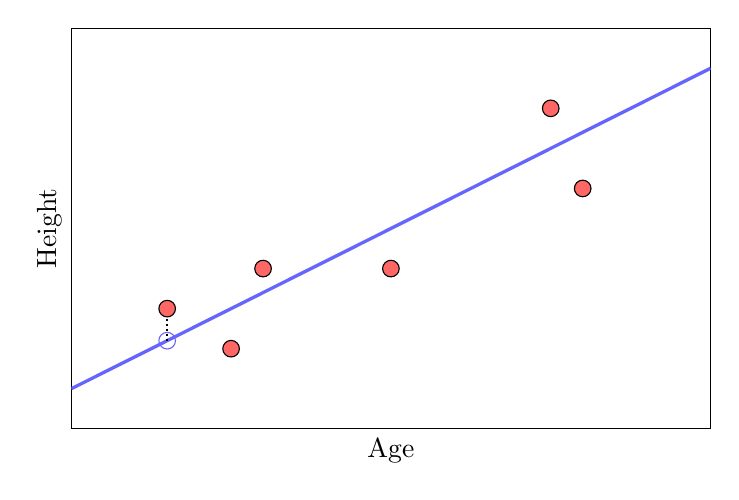
\begin{tikzpicture}
				\begin{axis}[
					xmin=0,
					xmax=1,
					ymin=0,
					ymax=1,
					ticks=none,
					xlabel=Age,
					ylabel=Height,
					height=0.55\textwidth,
					width=0.8\textwidth
				]

					\addplot[only marks, draw=black, fill=red!60, mark size=3pt] coordinates {
						(0.15, 0.3)
						(0.25, 0.2)
						(0.3, 0.4)
						(0.5, 0.4)
						(0.75, 0.8)
						(0.8, 0.6)
					};
					\addplot[blue!60, very thick] coordinates {
						(0, 0.1)
						(1, 0.9)
					};
					\addplot[only marks, mark=o, draw=blue!60, mark size=3pt] coordinates {
						(0.15, 0.1 + 0.15*0.8)
					};

					\addplot[densely dotted, thick] coordinates {
						(0.15, 0.3)
						(0.15, 0.1 + 0.15*0.8)
					};
				\end{axis}
			\end{tikzpicture}
		}
		\begin{tikzpicture}
			\node[] at (-5.3, 2.5) {};
			\node[] at (5.3, -5) {};
			\node[] at (0, 0) {
				\usebox{\boxthree}
			};
			\node[anchor=north] at (0, -2.5) {
				\begin{math}
					\begin{alignedat}{2}
						\hat{y} &= 0.9x + 0.1\\
					\end{alignedat}
				\end{math}
			};
		\end{tikzpicture}
	\end{frame}

	\begin{frame}{Training a neural network: Loss functions}
		\newsavebox{\boxtwo}
		\sbox{\boxtwo}{%
			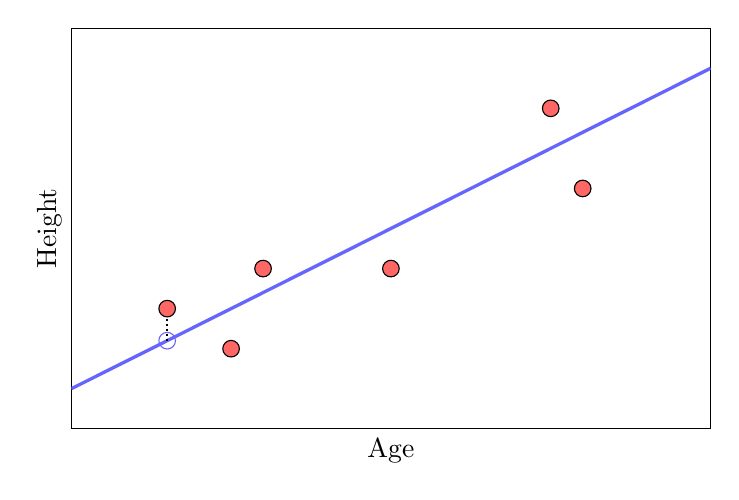
\begin{tikzpicture}
				\begin{axis}[
					xmin=0,
					xmax=1,
					ymin=0,
					ymax=1,
					ticks=none,
					xlabel=Age,
					ylabel=Height,
					height=0.55\textwidth,
					width=0.8\textwidth
				]

					\addplot[only marks, draw=black, fill=red!60, mark size=3pt] coordinates {
						(0.15, 0.3)
						(0.25, 0.2)
						(0.3, 0.4)
						(0.5, 0.4)
						(0.75, 0.8)
						(0.8, 0.6)
					};
					\addplot[blue!60, very thick] coordinates {
						(0, 0.1)
						(1, 0.9)
					};
					\addplot[only marks, mark=o, draw=blue!60, mark size=3pt] coordinates {
						(0.15, 0.1 + 0.15*0.8)
					};

					\addplot[densely dotted, thick] coordinates {
						(0.15, 0.3)
						(0.15, 0.1 + 0.15*0.8)
					};
				\end{axis}
			\end{tikzpicture}
		}
		\begin{tikzpicture}
			\node[] at (-5.3, 2.5) {};
			\node[] at (5.3, -5) {};
			\node[] at (0, 0) {
				\usebox{\boxtwo}
			};
			\node[anchor=north] at (-0.37, -2.5) {
				\begin{math}
					\begin{alignedat}{2}
						\hat{y} &= 0.9x + 0.1\\
						error_i &= |\hat{y}-y|\\
					\end{alignedat}
				\end{math}
			};
		\end{tikzpicture}
	\end{frame}

	\begin{frame}{Training a neural network: Loss functions}
		\newsavebox{\boxone}
		\sbox{\boxone}{%
			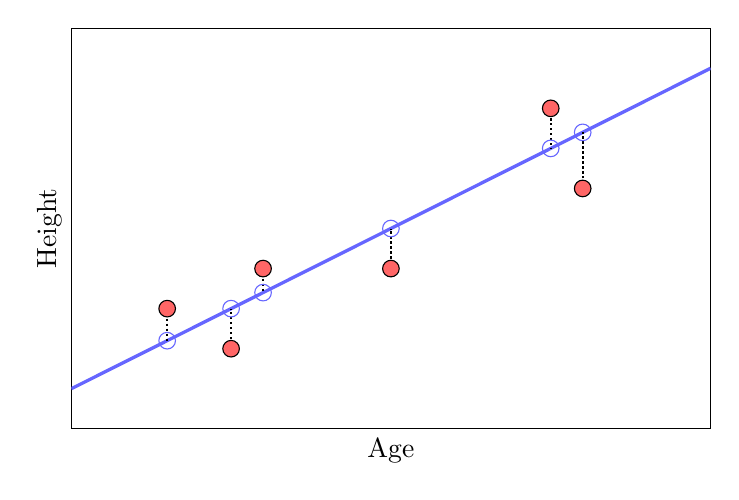
\begin{tikzpicture}
				\begin{axis}[
					xmin=0,
					xmax=1,
					ymin=0,
					ymax=1,
					ticks=none,
					xlabel=Age,
					ylabel=Height,
					height=0.55\textwidth,
					width=0.8\textwidth
				]

					\addplot[only marks, draw=black, fill=red!60, mark size=3pt] coordinates {
						(0.15, 0.3)
						(0.25, 0.2)
						(0.3, 0.4)
						(0.5, 0.4)
						(0.75, 0.8)
						(0.8, 0.6)
					};
					\addplot[blue!60, very thick] coordinates {
						(0, 0.1)
						(1, 0.9)
					};
					\addplot[only marks, mark=o, draw=blue!60, mark size=3pt] coordinates {
						(0.15, 0.1 + 0.15*0.8)
						(0.25, 0.1 + 0.25*0.8)
						(0.3, 0.1 + 0.3*0.8)
						(0.5, 0.1 + 0.5*0.8)
						(0.75, 0.1 + 0.75*0.8)
						(0.8, 0.1 + 0.8*0.8)
					};

					\addplot[densely dotted, thick] coordinates {
						(0.15, 0.3)
						(0.15, 0.1 + 0.15*0.8)
					};

					\addplot[densely dotted, thick] coordinates {
						(0.25, 0.2)
						(0.25, 0.1 + 0.25*0.8)
					};

					\addplot[densely dotted, thick] coordinates {
						(0.3, 0.4)
						(0.3, 0.1 + 0.3*0.8)
					};

					\addplot[densely dotted, thick] coordinates {
						(0.5, 0.4)
						(0.5, 0.1 + 0.5*0.8)
					};

					\addplot[densely dotted, thick] coordinates {
						(0.75, 0.8)
						(0.75, 0.1 + 0.75*0.8)
					};

					\addplot[densely dotted, thick] coordinates {
						(0.8, 0.6)
						(0.8, 0.1 + 0.8*0.8)
					};
				\end{axis}
			\end{tikzpicture}
		}
		\begin{tikzpicture}
			\node[] at (-5.3, 2.5) {};
			\node[] at (5.3, -5) {};
			\node[] at (0, 0) {
				\usebox{\boxone}
			};
			\node[anchor=north] at (0, -2.5) {
				\begin{math}
					\begin{alignedat}{2}
						\hat{y} &= 0.9x + 0.1\\
						error_i &= |\hat{y}-y|\\
						mse &= \frac{1}{n}\sum\limits_{i<n} (\hat{y}_i-y_i)^2
					\end{alignedat}
				\end{math}
			};
		\end{tikzpicture}
	\end{frame}

	\begin{frame}{Training a neural network: Gradient descent}
		\begin{tikzpicture}
			\node[] at (-5, 3) {};
			\node[] at (5, -4.5) {};

			\node[
				circle,
				draw=black,
				fill=green!20,
				minimum size=\nodesize,
				inner sep=0pt
			] (n) at (0, 1.5) {};

			\node[] (x) at (-1.5, 1.5) {$x$};
			\node[] (b) at (0, 2.5) {$0.1$};
			\node[] (y) at (1.5, 1.5) {$y$};
			\node[] at (0, 0) {$y=0.4x+0.1$\hspace*{0.75cm}$loss=(y-\hat{y})^2$};

			\draw[->] (x) -- (n) node [midway, above] {$0.4$};
			\draw[->] (b) -- (n);
			\draw[->] (n) -- (y);
		\end{tikzpicture}
	\end{frame}

	\begin{frame}{Training a neural network: Gradient descent}
		\begin{tikzpicture}
			\node[] at (-5, 3) {};
			\node[] at (5, -4.5) {};

			\node[
				circle,
				draw=black,
				fill=green!20,
				minimum size=\nodesize,
				inner sep=0pt
			] (n) at (0, 1.5) {};

			\node[] (x) at (-1.5, 1.5) {$x$};
			\node[] (b) at (0, 2.5) {$0.1$};
			\node[] (y) at (1.5, 1.5) {$y$};
			\node[] at (0, 0) {$0.16=0.4*0.15+0.1$\hspace*{0.75cm}$0.019=(0.3-0.16)^2$};

			\draw[->] (x) -- (n) node [midway, above] {$0.4$};
			\draw[->] (b) -- (n);
			\draw[->] (n) -- (y);
		\end{tikzpicture}
	\end{frame}

	\begin{frame}{Training a neural network: Gradient descent}
		\begin{tikzpicture}
			\node[] at (-5, 3) {};
			\node[] at (5, -4.5) {};

			\node[
				circle,
				draw=black,
				fill=green!20,
				minimum size=\nodesize,
				inner sep=0pt
			] (n) at (0, 1.5) {};

			\node[] (x) at (-1.5, 1.5) {$x$};
			\node[] (b) at (0, 2.5) {$0.1$};
			\node[] (y) at (1.5, 1.5) {$y$};
			\node[] at (0, 0) {$(0.3 - (0.4*0.15+0.1))^2=0.019$};

			\draw[->] (x) -- (n) node [midway, above] {$0.4$};
			\draw[->] (b) -- (n);
			\draw[->] (n) -- (y);
		\end{tikzpicture}
	\end{frame}

	\begin{frame}{Training a neural network: Gradient descent}
		\begin{tikzpicture}
			\node[] at (-5, 3) {};
			\node[] at (5, -4.5) {};

			\node[
				circle,
				draw=black,
				fill=green!20,
				minimum size=\nodesize,
				inner sep=0pt
			] (n) at (0, 1.5) {};

			\node[] (x) at (-1.5, 1.5) {$x$};
			\node[] (b) at (0, 2.5) {$0.1$};
			\node[] (y) at (1.5, 1.5) {$y$};
			\node[] at (0, 0) {$(0.3 - (0.4*0.15+0.1))^2=0.019$};

			\draw[->] (x) -- (n) node [midway, above] {$0.4$};
			\draw[->] (b) -- (n);
			\draw[->] (n) -- (y);

			\node[] at (-2.4, -0.6) {\footnotesize{\textcolor{red}{$y$}}};
			\draw[->, red] (-2.4, -0.4) -- (-2.4, -0.2);
			\node[] at (-0.35, -0.6) {\footnotesize{\textcolor{red}{$\hat{y}$}}};
			\draw[->, red] (-0.35, -0.4) -- (-0.35, -0.2);
			\draw[red] (-1.55, -0.15) -- (0.95, -0.15);
			\node[] at (-0.35, 0.6) {\footnotesize{\textcolor{red}{$x$}}};
			\draw[->, red] (-0.35, 0.4) -- (-0.35, 0.2);
			\node[] at (-1.27, 0.6) {\footnotesize{\textcolor{red}{$w$}}};
			\draw[->, red] (-1.27, 0.4) -- (-1.27, 0.2);
			\node[] at (0.75, 0.6) {\footnotesize{\textcolor{red}{$b$}}};
			\draw[->, red] (0.75, 0.4) -- (0.75, 0.2);
			\node[] at (2.4, 0.6) {\footnotesize{\textcolor{red}{$loss$}}};
			\draw[->, red] (2.4, 0.4) -- (2.4, 0.2);
		\end{tikzpicture}
	\end{frame}

	\begin{frame}{Training a neural network: Gradient descent}
		\newsavebox{\lossboxtwo}
		\sbox{\lossboxtwo}{%
			\begin{tikzpicture}
				\begin{axis}[
					ticks=none,
					ymin=0,
					ymax=0.025,
					xmin=0,
					xmax=2,
					height=4cm,
					width=5cm,
					ylabel=$loss$,
					xlabel=$w$
				]
					\addplot[only marks, draw=black, fill=purple!60] coordinates {
						(0.4, 0.019)
					};
				\end{axis}
			\end{tikzpicture}
		}
		\begin{tikzpicture}
			\node[] at (-5, 3) {};
			\node[] at (5, -4.5) {};

			\node[
				circle,
				draw=black,
				fill=green!20,
				minimum size=\nodesize,
				inner sep=0pt
			] (n) at (0, 1.5) {};

			\node[] (x) at (-1.5, 1.5) {$x$};
			\node[] (b) at (0, 2.5) {$0.1$};
			\node[] (y) at (1.5, 1.5) {$y$};
			\node[] at (0, 0) {$(0.3 - (0.4*0.15+0.1))^2=0.019$};

			\draw[->] (x) -- (n) node [midway, above] {$0.4$};
			\draw[->] (b) -- (n);
			\draw[->] (n) -- (y);

			\node[] at (0, -2.5) {
				\usebox{\lossboxtwo}
			};

		\end{tikzpicture}
	\end{frame}

	\begin{frame}{Training a neural network: Gradient descent}
		\newsavebox{\lossboxone}
		\sbox{\lossboxone}{%
			\begin{tikzpicture}
				\begin{axis}[
					ticks=none,
					ymin=0,
					ymax=0.025,
					xmin=0,
					xmax=2,
					height=4cm,
					width=5cm,
					ylabel=$loss$,
					xlabel=$w$
				]
					\addplot[only marks, draw=black, fill=purple!60] coordinates {
						(0.9, 0.004)
						(0.4, 0.019)
					};
				\end{axis}
			\end{tikzpicture}
		}
		\begin{tikzpicture}
			\node[] at (-5, 3) {};
			\node[] at (5, -4.5) {};

			\node[
				circle,
				draw=black,
				fill=green!20,
				minimum size=\nodesize,
				inner sep=0pt
			] (n) at (0, 1.5) {};

			\node[] (x) at (-1.5, 1.5) {$x$};
			\node[] (b) at (0, 2.5) {$0.1$};
			\node[] (y) at (1.5, 1.5) {$y$};
			\node[] at (0, 0) {$(0.3 - (0.9*0.15+0.1))^2=0.004$};

			\draw[->] (x) -- (n) node [midway, above] {$0.9$};
			\draw[->] (b) -- (n);
			\draw[->] (n) -- (y);

			\node[] at (0, -2.5) {
				\usebox{\lossboxone}
			};

		\end{tikzpicture}
	\end{frame}

	\begin{frame}{Training a neural network: Gradient descent}
		\newsavebox{\lossbox}
		\sbox{\lossbox}{%
			\begin{tikzpicture}
				\begin{axis}[
					ticks=none,
					ymin=0,
					ymax=0.025,
					xmin=0,
					xmax=2,
					height=4cm,
					width=5cm,
					ylabel=$loss$,
					xlabel=$w$
				]
					\addplot[only marks, draw=black, fill=purple!60] coordinates {
						(0.9, 0.004)
						(0.4, 0.019)
					};
					\addplot[] table [x=x,y=y,col sep=comma]{notebooks/data.csv};
				\end{axis}
			\end{tikzpicture}
		}
		\begin{tikzpicture}
			\node[] at (-5, 3) {};
			\node[] at (5, -4.5) {};

			\node[
				circle,
				draw=black,
				fill=green!20,
				minimum size=\nodesize,
				inner sep=0pt
			] (n) at (0, 1.5) {};

			\node[] (x) at (-1.5, 1.5) {$x$};
			\node[] (b) at (0, 2.5) {$0.1$};
			\node[] (y) at (1.5, 1.5) {$y$};
			\node[] at (0, 0) {$(0.3 - (0.9*0.15+0.1))^2=0.004$};

			\draw[->] (x) -- (n) node [midway, above] {$0.9$};
			\draw[->] (b) -- (n);
			\draw[->] (n) -- (y);

			\node[] at (0, -2.5) {
				\usebox{\lossbox}
			};

		\end{tikzpicture}
	\end{frame}

	\begin{frame}{Training a neural network: Gradient descent}
		\newsavebox{\lossboxthree}
		\sbox{\lossboxthree}{%
			\begin{tikzpicture}
				\begin{axis}[
					ticks=none,
					ymin=0,
					ymax=0.025,
					xmin=0,
					xmax=2,
					height=4cm,
					width=5cm,
					ylabel=$loss$,
					xlabel=$w$
				]
					\addplot[only marks, draw=black, fill=purple!60] coordinates {
						(0.4, 0.019)
					};
					\addplot[] coordinates {
						(0.38, 0.021)
						(0.42, 0.017)
					};
				\end{axis}
			\end{tikzpicture}
		}

		\newsavebox{\boxeight}
		\sbox{\boxeight}{%
			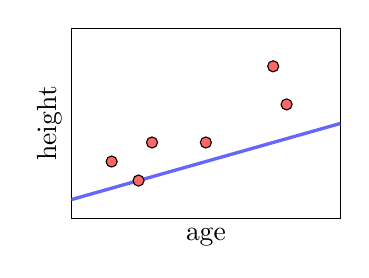
\begin{tikzpicture}
				\begin{axis}[
					xmin=0,
					xmax=1,
					ymin=0,
					ymax=1,
					ticks=none,
					xlabel=age,
					ylabel=height,
					height=4cm,
					width=5cm,
					xlabel style={text depth=0}
				]

					\addplot[only marks, draw=black, fill=red!60, mark size=2pt] coordinates {
						(0.15, 0.3)
						(0.25, 0.2)
						(0.3, 0.4)
						(0.5, 0.4)
						(0.75, 0.8)
						(0.8, 0.6)
					};
					\addplot[blue!60, very thick] coordinates {
						(0, 0.1)
						(1, 0.5)
					};
				\end{axis}
			\end{tikzpicture}
		}

		\begin{tikzpicture}
			\node[] at (-5, 3) {};
			\node[] at (5, -4.5) {};

			\node[
				circle,
				draw=black,
				fill=green!20,
				minimum size=\nodesize,
				inner sep=0pt
			] (n) at (0, 1.5) {};

			\node[] (x) at (-1.5, 1.5) {$x$};
			\node[] (b) at (0, 2.5) {$0.1$};
			\node[] (y) at (1.5, 1.5) {$y$};
			\node[] at (0, 0) {$(0.3 - (0.4*0.15+0.1))^2=0.019$};

			\draw[->] (x) -- (n) node [midway, above] {$0.4$};
			\draw[->] (b) -- (n);
			\draw[->] (n) -- (y);

			\node[] at (-2.5, -2.5) {
				\usebox{\lossboxthree}
			};

			\node[] at (2.5, -2.5) {
				\usebox{\boxeight}
			};

		\end{tikzpicture}
	\end{frame}

	\begin{frame}{Training a neural network: Gradient descent}
		\newsavebox{\lossboxfour}
		\sbox{\lossboxfour}{%
			\begin{tikzpicture}
				\begin{axis}[
					ticks=none,
					ymin=0,
					ymax=0.025,
					xmin=0,
					xmax=2,
					height=4cm,
					width=5cm,
					ylabel=$loss$,
					xlabel=$w$,
					clip=false
				]
					\addplot[only marks, draw=black, fill=purple!60] coordinates {
						(0.4, 0.019)
					};
					\addplot[] coordinates {
						(0.38, 0.021)
						(0.42, 0.017)
					};
					\draw[->] (axis cs: 0.4, 0.019) -- (axis cs: 1.7, 0.019);
					\addplot[dashed] coordinates {
						(1.7, 0.025)
						(1.7, 0)
					};
					\node[anchor=north] at (axis cs: 1.7, 0) {\footnotesize{1.7}};
				\end{axis}
			\end{tikzpicture}
		}

		\newsavebox{\boxnine}
		\sbox{\boxnine}{%
			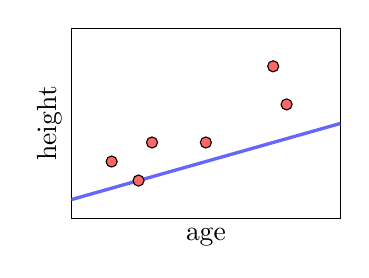
\begin{tikzpicture}
				\begin{axis}[
					xmin=0,
					xmax=1,
					ymin=0,
					ymax=1,
					ticks=none,
					xlabel=age,
					ylabel=height,
					height=4cm,
					width=5cm,
					xlabel style={text depth=0}
				]

					\addplot[only marks, draw=black, fill=red!60, mark size=2pt] coordinates {
						(0.15, 0.3)
						(0.25, 0.2)
						(0.3, 0.4)
						(0.5, 0.4)
						(0.75, 0.8)
						(0.8, 0.6)
					};
					\addplot[blue!60, very thick] coordinates {
						(0, 0.1)
						(1, 0.5)
					};
				\end{axis}
			\end{tikzpicture}
		}

		\begin{tikzpicture}
			\node[] at (-5, 3) {};
			\node[] at (5, -4.5) {};

			\node[
				circle,
				draw=black,
				fill=green!20,
				minimum size=\nodesize,
				inner sep=0pt
			] (n) at (0, 1.5) {};

			\node[] (x) at (-1.5, 1.5) {$x$};
			\node[] (b) at (0, 2.5) {$0.1$};
			\node[] (y) at (1.5, 1.5) {$y$};
			\node[] at (0, 0) {$(0.3 - (0.4*0.15+0.1))^2=0.019$};

			\draw[->] (x) -- (n) node [midway, above] {$0.4$};
			\draw[->] (b) -- (n);
			\draw[->] (n) -- (y);

			\node[] at (-2.5, -2.5) {
				\usebox{\lossboxfour}
			};

			\node[] at (2.5, -2.5) {
				\usebox{\boxnine}
			};

		\end{tikzpicture}
	\end{frame}

	\begin{frame}{Training a neural network: Gradient descent}
		\newsavebox{\lossboxfive}
		\sbox{\lossboxfive}{%
			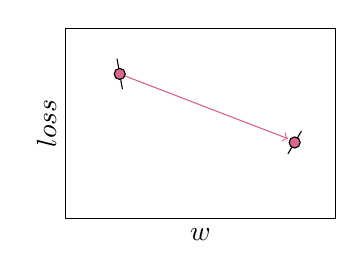
\begin{tikzpicture}
				\begin{axis}[
					ticks=none,
					ymin=0,
					ymax=0.025,
					xmin=0,
					xmax=2,
					height=4cm,
					width=5cm,
					ylabel=$loss$,
					xlabel=$w$,
					clip=false
				]
					\addplot[only marks, draw=black, fill=purple!60] coordinates {
						(0.4, 0.019)
						(1.7, 0.01)
					};

					\addplot[] coordinates {
						(0.38, 0.021)
						(0.42, 0.017)
					};

					\addplot[] coordinates {
						(1.75, 0.0115)
						(1.65, 0.0085)
					};

					\draw[->,purple!60] (axis cs: 0.4, 0.019) -- (axis cs: 1.65, 0.0105);

				\end{axis}
			\end{tikzpicture}
		}

		\newsavebox{\boxten}
		\sbox{\boxten}{%
			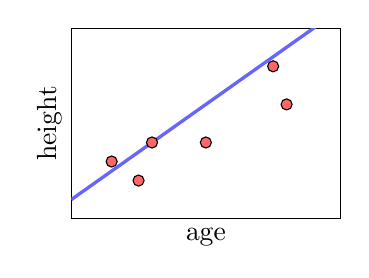
\begin{tikzpicture}
				\begin{axis}[
					xmin=0,
					xmax=1,
					ymin=0,
					ymax=1,
					ticks=none,
					xlabel=age,
					ylabel=height,
					height=4cm,
					width=5cm,
					xlabel style={text depth=0}
				]

					\addplot[only marks, draw=black, fill=red!60, mark size=2pt] coordinates {
						(0.15, 0.3)
						(0.25, 0.2)
						(0.3, 0.4)
						(0.5, 0.4)
						(0.75, 0.8)
						(0.8, 0.6)
					};
					\addplot[blue!60, very thick] coordinates {
						(0, 0.1)
						(1, 1.1)
					};
				\end{axis}
			\end{tikzpicture}
		}

		\begin{tikzpicture}
			\node[] at (-5, 3) {};
			\node[] at (5, -4.5) {};

			\node[
				circle,
				draw=black,
				fill=green!20,
				minimum size=\nodesize,
				inner sep=0pt
			] (n) at (0, 1.5) {};

			\node[] (x) at (-1.5, 1.5) {$x$};
			\node[] (b) at (0, 2.5) {$0.1$};
			\node[] (y) at (1.5, 1.5) {$y$};
			\node[] at (0, 0) {$(0.3 - ($\textcolor{red}{$1.7$}$*0.15+0.1))^2=0.003$};

			\draw[->, red] (x) -- (n) node [midway, above] {\textcolor{red}{$1.7$}};
			\draw[->] (b) -- (n);
			\draw[->] (n) -- (y);

			\node[] at (-2.5, -2.5) {
				\usebox{\lossboxfive}
			};

			\node[] at (2.5, -2.5) {
				\usebox{\boxten}
			};

		\end{tikzpicture}
	\end{frame}

	\begin{frame}{Training a neural network: Gradient descent}
		\newsavebox{\lossboxsix}
		\sbox{\lossboxsix}{%
			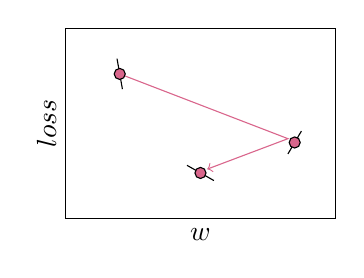
\begin{tikzpicture}
				\begin{axis}[
					ticks=none,
					ymin=0,
					ymax=0.025,
					xmin=0,
					xmax=2,
					height=4cm,
					width=5cm,
					ylabel=$loss$,
					xlabel=$w$,
					clip=false
				]
					\addplot[only marks, draw=black, fill=purple!60] coordinates {
						(0.4, 0.019)
						(1.7, 0.01)
						(1.0, 0.006)
					};

					\addplot[] coordinates {
						(0.38, 0.021)
						(0.42, 0.017)
					};

					\addplot[] coordinates {
						(1.75, 0.0115)
						(1.65, 0.0085)
					};

					\addplot[] coordinates {
						(0.9, 0.007)
						(1.1, 0.005)
					};

					\draw[->,purple!60] (axis cs: 0.4, 0.019) --
										(axis cs: 1.65, 0.0105) --
										(axis cs: 1.05, 0.0065);

				\end{axis}
			\end{tikzpicture}
		}

		\newsavebox{\boxeleven}
		\sbox{\boxeleven}{%
			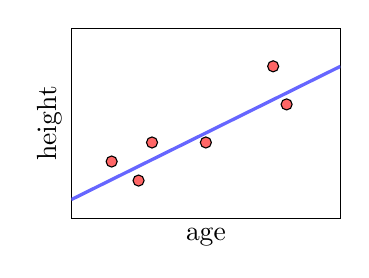
\begin{tikzpicture}
				\begin{axis}[
					xmin=0,
					xmax=1,
					ymin=0,
					ymax=1,
					ticks=none,
					xlabel=age,
					ylabel=height,
					height=4cm,
					width=5cm,
					xlabel style={text depth=0}
				]

					\addplot[only marks, draw=black, fill=red!60, mark size=2pt] coordinates {
						(0.15, 0.3)
						(0.25, 0.2)
						(0.3, 0.4)
						(0.5, 0.4)
						(0.75, 0.8)
						(0.8, 0.6)
					};
					\addplot[blue!60, very thick] coordinates {
						(0, 0.1)
						(1, 0.8)
					};
				\end{axis}
			\end{tikzpicture}
		}

		\begin{tikzpicture}
			\node[] at (-5, 3) {};
			\node[] at (5, -4.5) {};

			\node[
				circle,
				draw=black,
				fill=green!20,
				minimum size=\nodesize,
				inner sep=0pt
			] (n) at (0, 1.5) {};

			\node[] (x) at (-1.5, 1.5) {$x$};
			\node[] (b) at (0, 2.5) {$0.1$};
			\node[] (y) at (1.5, 1.5) {$y$};
			\node[] at (0, 0) {$(0.3 - ($\textcolor{red}{$1.0$}$*0.15+0.1))^2=0.002$};

			\draw[->, red] (x) -- (n) node [midway, above] {\textcolor{red}{$1.0$}};
			\draw[->] (b) -- (n);
			\draw[->] (n) -- (y);

			\node[] at (-2.5, -2.5) {
				\usebox{\lossboxsix}
			};

			\node[] at (2.5, -2.5) {
				\usebox{\boxeleven}
			};

		\end{tikzpicture}
	\end{frame}

	\begin{frame}{Training a neural network: Gradient descent}
		\newsavebox{\lossboxseven}
		\sbox{\lossboxseven}{%
			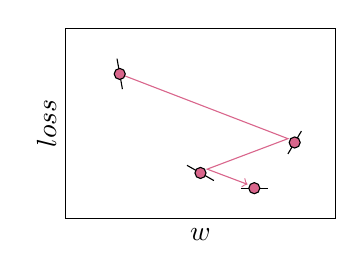
\begin{tikzpicture}
				\begin{axis}[
					ticks=none,
					ymin=0,
					ymax=0.025,
					xmin=0,
					xmax=2,
					height=4cm,
					width=5cm,
					ylabel=$loss$,
					xlabel=$w$,
					clip=false,
				]
					\addplot[only marks, draw=black, fill=purple!60] coordinates {
						(0.4, 0.019)
						(1.7, 0.01)
						(1.0, 0.006)
						(1.4, 0.004)
					};

					\addplot[] coordinates {
						(0.38, 0.021)
						(0.42, 0.017)
					};

					\addplot[] coordinates {
						(1.75, 0.0115)
						(1.65, 0.0085)
					};

					\addplot[] coordinates {
						(0.9, 0.007)
						(1.1, 0.005)
					};

					\addplot[] coordinates {
						(1.3, 0.004)
						(1.5, 0.004)
					};

					\draw[->,purple!60] (axis cs: 0.4, 0.019) --
										(axis cs: 1.65, 0.0105) --
										(axis cs: 1.05, 0.0065) --
										(axis cs: 1.35, 0.0045);

				\end{axis}
			\end{tikzpicture}
		}

		\newsavebox{\boxtwelve}
		\sbox{\boxtwelve}{%
			\begin{tikzpicture}
				\begin{axis}[
					xmin=0,
					xmax=1,
					ymin=0,
					ymax=1,
					ticks=none,
					xlabel=age,
					ylabel=height,
					height=4cm,
					width=5cm,
					xlabel style={text depth=0}
				]

					\addplot[only marks, draw=black, fill=red!60, mark size=2pt] coordinates {
						(0.15, 0.3)
						(0.25, 0.2)
						(0.3, 0.4)
						(0.5, 0.4)
						(0.75, 0.8)
						(0.8, 0.6)
					};
					\addplot[blue!60, very thick] coordinates {
						(0, 0.1)
						(1, 0.9)
					};
				\end{axis}
			\end{tikzpicture}
		}

		\begin{tikzpicture}
			\node[] at (-5, 3) {};
			\node[] at (5, -4.5) {};

			\node[
				circle,
				draw=black,
				fill=green!20,
				minimum size=\nodesize,
				inner sep=0pt
			] (n) at (0, 1.5) {};

			\node[] (x) at (-1.5, 1.5) {$x$};
			\node[] (b) at (0, 2.5) {$0.1$};
			\node[] (y) at (1.5, 1.5) {$y$};
			\node[] at (0, 0) {$(0.3 - ($\textcolor{red}{$1.2$}$*0.15+0.1))^2=0.000$};

			\draw[->, red] (x) -- (n) node [midway, above] {\textcolor{red}{$1.2$}};
			\draw[->] (b) -- (n);
			\draw[->] (n) -- (y);

			\node[] at (-2.5, -2.5) {
				\usebox{\lossboxseven}
			};

			\node[] at (2.5, -2.5) {
				\usebox{\boxtwelve}
			};

		\end{tikzpicture}
	\end{frame}

	\begin{frame}{Training a neural network: Summary}
		\centering
		\vfill
		\begin{itemize}
			\item The loss function is a mathematical formalization of what we want the model to learn
			\item Calculating the gradient allows us to see how we can update the parameters of the model to decrease the loss
			\item Using gradient descent we can update the parameters sequentially until we have the perfect model with zero loss
		\end{itemize}
		\vfill
	\end{frame}
\end{document}
